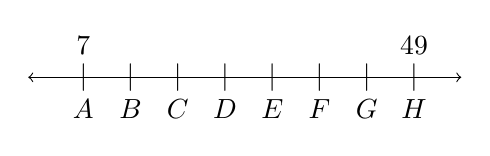
\begin{tikzpicture}
\draw[<->](0,0)--(5.5,0);
\draw(.7,0)node{$|$}(1.3,0)node{$|$}(1.9,0)node{$|$}(2.5,0)node{$|$}(3.1,0)node{$|$}(3.7,0)node{$|$}(4.3,0)node{$|$}(4.9,0)node{$|$};
\draw(.7,-.4)node{$A$}(1.3,-.4)node{$B$}(1.9,-.4)node{$C$}(2.5,-.4)node{$D$}(3.1,-.4)node{$E$}(3.7,-.4)node{$F$}(4.3,-.4)node{$G$}(4.9,-.4)node{$H$};
\draw(.7,.4)node{$7$}(4.9,.4)node{$49$};
\end{tikzpicture}

On the number line above, all the intervals between points are the same.  Point $A$ is at $7$ and point $H$ is at $49$.  What is the coordinate of $C$?



\ifsat
	\begin{enumerate}[label=\Alph*)]
		\item $6$
		\item $12$
		\item $13$
		\item $19$%
	\end{enumerate}
\else
\fi

\ifacteven
	\begin{enumerate}[label=\textbf{\Alph*.},itemsep=\fill,align=left]
		\setcounter{enumii}{5}
		\item $6$
		\item $12$
		\item $13$
		\addtocounter{enumii}{1}
		\item $14$
		\item $19$%
	\end{enumerate}
\else
\fi

\ifactodd
	\begin{enumerate}[label=\textbf{\Alph*.},itemsep=\fill,align=left]
		\item $6$
		\item $12$
		\item $13$
		\item $14$
		\item $19$%
	\end{enumerate}
\else
\fi

\ifgridin
 $19$%

\else
\fi

